% -----------------------------------------------------------------------------
\section{Conventions}
% -----------------------------------------------------------------------------

This section provides some preliminary information to aid in the understanding of the specification.
The SBOL data model is specified using Unified Modeling Language (UML) 2.0 diagrams \href{http://www.omg.org/spec/UML/2.0/}{(OMG 2005)}. This section reviews terminology conventions, the basics of UML diagrams, and our naming conventions.

\subsection{Terminology Conventions}

This document indicates requirement levels using the controlled vocabulary specified in \href{https://tools.ietf.org/html/rfc2119}{IETF RFC 2119}.
In particular, the key words ``MUST'', ``MUST NOT'', ``REQUIRED'', ``SHALL'', ``SHALL NOT'', ``SHOULD'', ``SHOULD NOT'', ``RECOMMENDED'', ``MAY'', and ``OPTIONAL'' in this document are to be interpreted as described in RFC 2119.

\begin{itemize}
\item The words ``MUST'', ``REQUIRED'', or ``SHALL'' mean that the item is an absolute requirement.
\item The phrases ``MUST NOT'' or ``SHALL NOT'' mean that the item is an absolute prohibition.
\item The word ``SHOULD'' or the adjective ``RECOMMENDED'' mean that there might exist valid reasons in particular circumstances to ignore a particular item, but the full implications need to be understood and carefully weighed before choosing a different course.
\item The phrases ``SHOULD NOT'' or ``NOT RECOMMENDED'' mean that there might exist valid reasons in particular circumstances when the particular behavior is acceptable or even useful, but the full implications needs to be understood and the case carefully weighed before implementing any behavior described with this label.
\item The word ``MAY'' or the adjective ``OPTIONAL'' mean that an item is truly optional.
\end{itemize}

\subsection{UML Diagram Conventions}
\label{sec:umldiagrams}

The types of biological design data modeled by SBOL are commonly referred to as {\em classes}, especially when discussing the details of software implementation. Each SBOL class can be instantiated by many SBOL objects. These objects MAY contain data that differ in content, but they MUST agree on the type and form of their data as dictated by their common class. Classes are represented in UML diagrams as rectangles labeled at the top with class names (see \ref{fig:uml_sampler} for examples).

\begin{figure}[ht]
\begin{center}
  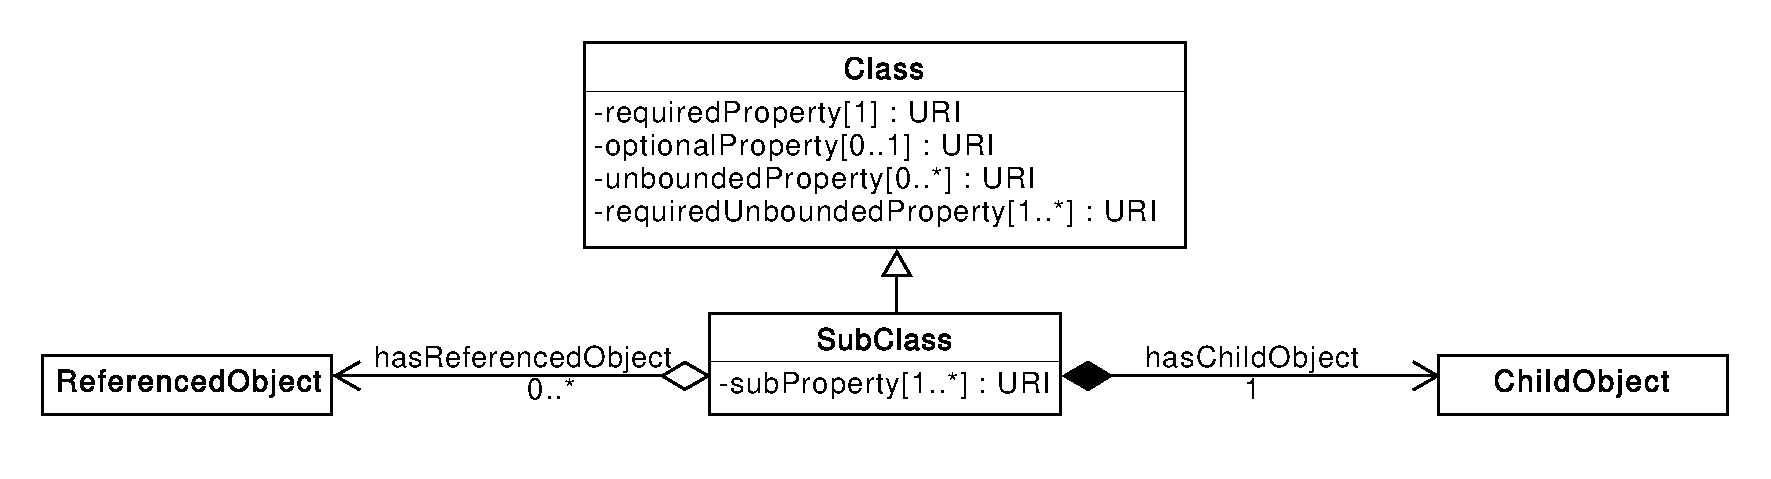
\includegraphics[width=\textwidth]{uml/uml_sampler.pdf}
\caption{Examples of UML diagram conventions used in this document}
\label{fig:uml_sampler}
\end{center}
\end{figure}

Classes can be connected to other classes by association properties, which are represented in UML diagrams as arrows. These arrows are labeled with data cardinalities in order to indicate how many values a given association property can possess (see below). The remaining (non-association) properties of a class are listed below its name. Each of the latter properties is labeled with its data type and cardinality.

In the case of an association property, the class from which the arrow originates is the owner of the association property. A diamond at the origin of the arrow indicates the type of association.
Open-faced diamonds indicate shared aggregation, also known as a reference, in which the owner of the association property exists independently of its value.

By contrast, filled diamonds indicate composite aggregation, also known as a part-whole relationship, in which the value of the association property MUST NOT exist independently of its owner.
In addition, in the SBOL data model, it is REQUIRED that the value of each composite aggregation property is a unique SBOL object (that is, not the value for more than one such property).
Note that in all cases, composite aggregation is used in such a way that there SHOULD NOT be duplication of such objects.
Such objects are also commonly referred to as ``child'' objects, and their owning objects as ``parent'' objects.

All SBOL properties are labeled with one of several restrictions on data cardinality. These are:

\begin{itemize}

\item $1$ - REQUIRED, one: there MUST be exactly one value for this property.

\item $0 \ldots 1$ - OPTIONAL: there MAY be a single value for this property, or it MAY be absent.

\item $0 \ldots *$ - unbounded: there MAY be any number of values for this property, including none.

\item $1 \ldots *$ - REQUIRED, unbounded: there MAY be any number of values for this property, as long as there is at least one.

\item $n \ldots *$ - at least: there MUST be at least $n$ values for this property.

\end{itemize}

Finally, classes can inherit the properties of other classes. Inheritance relationships are represented in UML diagrams as open-faced, triangular arrows that point from the inheriting class to the inherited class. Some classes in the SBOL data model cannot be instantiated as objects and exist only to group common properties for inheritance. These classes have italicized names and are known as abstract classes.

\subsection{Naming and Typographic Conventions}
\label{sec:nameconventions}

SBOL classes are named using upper ``camel case,'' meaning that each word is capitalized and all words are run together without spaces, e.g., \sbol{Identified}, \sbol{SequenceFeature}.
Properties, on the other hand, are named using lower camel case, meaning that they begin lowercase (e.g., \sbolmult{role:C}{role}) but if they consist of multiple words, all words after the first begin with an uppercase letter (e.g., \sbol{roleIntegration}).
SBOL properties are always given singular names irrespective of their cardinality, e.g., \sbolmult{role:C}{role} is used rather than \sbolmult{role:C}{role} even though a component can have multiple roles.
This is because each relation can potentially stand on its own, irrespective of the existence of others in the set.


% -----------------------------------------------------------------------------
\section{Identifiers and Primitive Types}
% -----------------------------------------------------------------------------

\subsection{Uniform Resource Identifiers}
\label{sec:URIstructure}

As SBOL is built upon the Resource Description Framework (RDF), all class instances are identified by a Uniform Resource Identifier (URI).  In the SBOL data model, the value of an association property MUST be a \sbol{URI} or set of \sbol{URI}s that refer to SBOL objects belonging to the class at the tip of the arrow.  Every \sbol{Identified} object's URI MUST be globally unique among all other \sbol{Identified} object URIs. It is also highly RECOMMENDED that the \sbol{URI} structure follows the recommended best practices for compliant \sbol{URI}s specified in \ref{sec:compliant}.

Whenever a \sbol{TopLevel} object's URI is a URL (e.g., following the conventions of HTTP(S) rather than a UUID), its structure MUST comply with the following rules:

\begin{itemize}

 \item A \sbol{TopLevel} URL MUST use the following pattern:
  \texttt{[namespace]/[local]/[displayId]},  where \texttt{namespace} and \sbol{displayId} are required fragments, and the \texttt{local} fragment is an optional relative path.
  	For example, a \sbol{Component} might have the URL~\path{https://synbiohub.org/public/igem/BBa_J23070}, where \texttt{namespace} is \path{https://synbiohub.org}, \texttt{local} is \path{public/igem}, and \texttt{displayId} is \path{BBa_J23070}.

  \item A \sbol{TopLevel} object's URL MUST NOT be included as prefix for any other \sbol{TopLevel} object (except for its controlling \sbol{Namespace}).
  	For example, the \path{BBa_J23070_seq} \sbol{Sequence} object cannot have a URL of \path{https://synbiohub.org/public/igem/BBa_J23070/BBa_J23070_seq}, since the\\ \path{https://synbiohub.org/public/igem/BBa_J23070} prefix is already used as a URL for the \path{BBa_J23070} \sbol{Component} object.

  \item The URL of any child or nested object MUST use the following pattern:\texttt{[parent]/[displayId]}, where \texttt{parent} is the URL of its parent object.
	Multiple layers of child objects are allowed using the same\\ \texttt{[parent]/[displayId]} pattern recursively.
	For example, a \sbol{SequenceFeature} object owned by the \path{BBa_J23070} \sbol{Component} and having a \sbol{displayId} of \texttt{annotation1} will have a URL of \path{https://synbiohub.org/public/igem/BBa_J23070/annotation1}.
	Similarly, the \texttt{loc1} \sbol{Location} child of the \texttt{annotation1}\\ \sbol{SequenceFeature} object will have the URL\\ \path{https://synbiohub.org/public/igem/BBa_J23070/annotation1/loc1}.
  \end{itemize}


\subsection{Primitive Data Types}
\label{sec:datatypes}
\label{sec:String}
\label{sec:Integer}
\label{sec:Long}
\label{sec:Double}
\label{sec:Boolean}
\label{sec:URI}
\label{sec:literal}

When SBOL uses simple ``primitive'' data types such as \sbol{String}s or \sbol{Integer}s, these are defined as the following specific formal types:
\begin{itemize}
\item \sbol{String}: \url{http://www.w3.org/TR/xmlschema11-2/#string}\\
  {\em Example: ``LacI coding sequence''}
\item \sbol{Integer}: \url{http://www.w3.org/TR/xmlschema11-2/#integer}\\
  {\em Example: 3}
\item \sbol{Long}: \url{http://www.w3.org/TR/xmlschema11-2/#long}\\
  {\em Example: 9223372036854775806}
\item \sbol{Double}: \url{http://www.w3.org/TR/xmlschema11-2/#double}\\
  {\em Example: 3.14159}
\item \sbol{Boolean}: \url{http://www.w3.org/TR/xmlschema11-2/#boolean}\\
  {\em Example: \external{true}}
\end{itemize}
The term \sbol{literal} is used to denote an object that can be any of the five types listed above.

In addition to the simple types listed above, SBOL also uses objects with types \emph{Uniform Resource Identifier} (\sbol{URI}). It is important to realize that in RDF, a \sbol{URI} might or might not be a resolvable URL (web address).  A \sbol{URI} is always a globally unique identifier within a structured namespace.  In some cases, that name is also a reference to (or within) a document, and in some cases that document can also be retrieved (e.g., using a web browser).
